%inputsCOPP_KGM-zwout-outputsP2_DX-3

\begin{figure}[htbp]
	\centering 
	\subfloat[P2 DX: Narx identification]{
		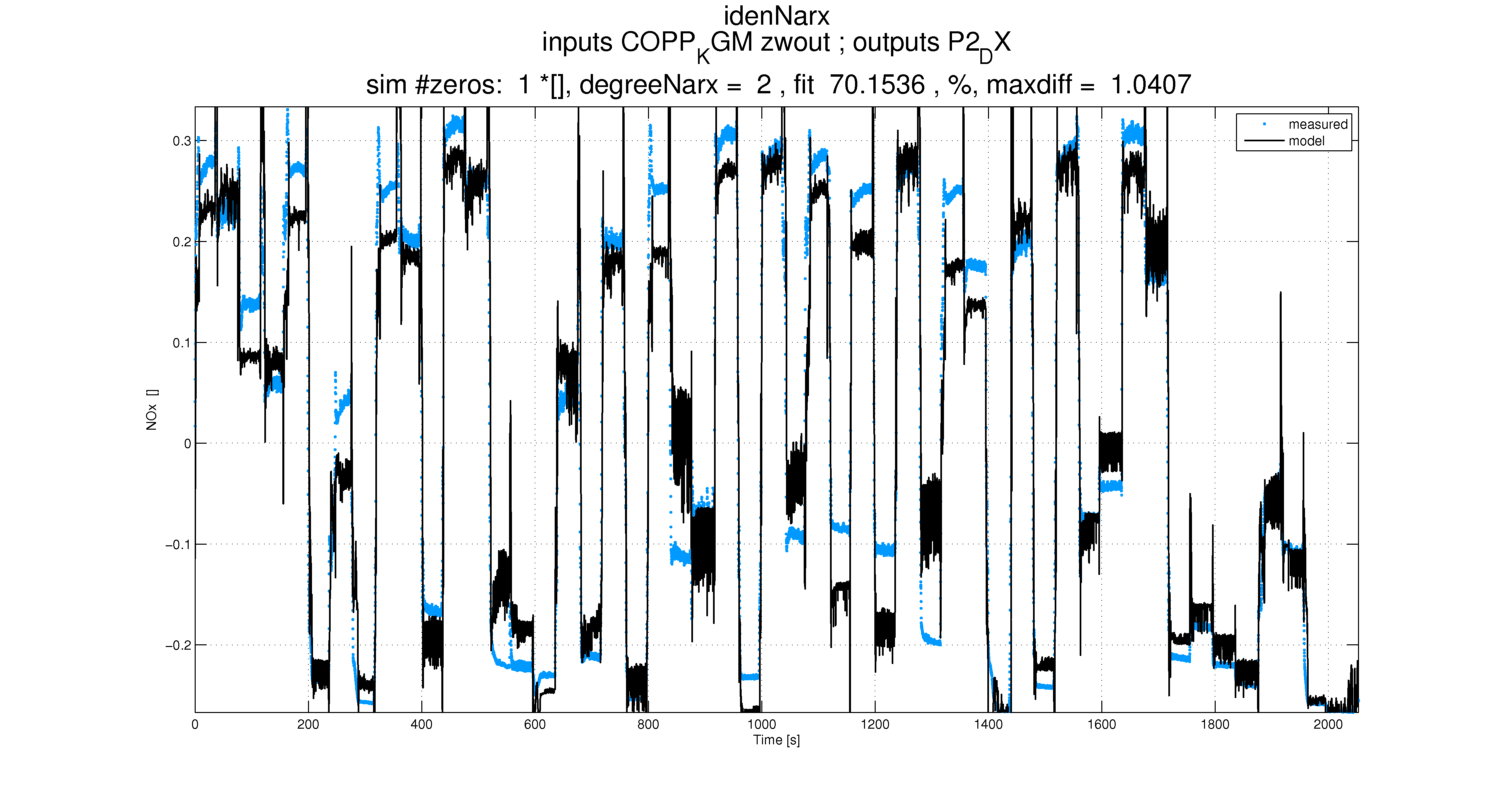
\includegraphics[width=.9\columnwidth]{Immagini/inputsCOPP_KGMzwoutoutputsP2_DX-idenNarx-3}
		\label{fig:inputsCOPP_KGMzwoutoutputsP2_DX-idenNarx-3}	}
	\\
	\subfloat[P2 DX: Narx prediction]{
		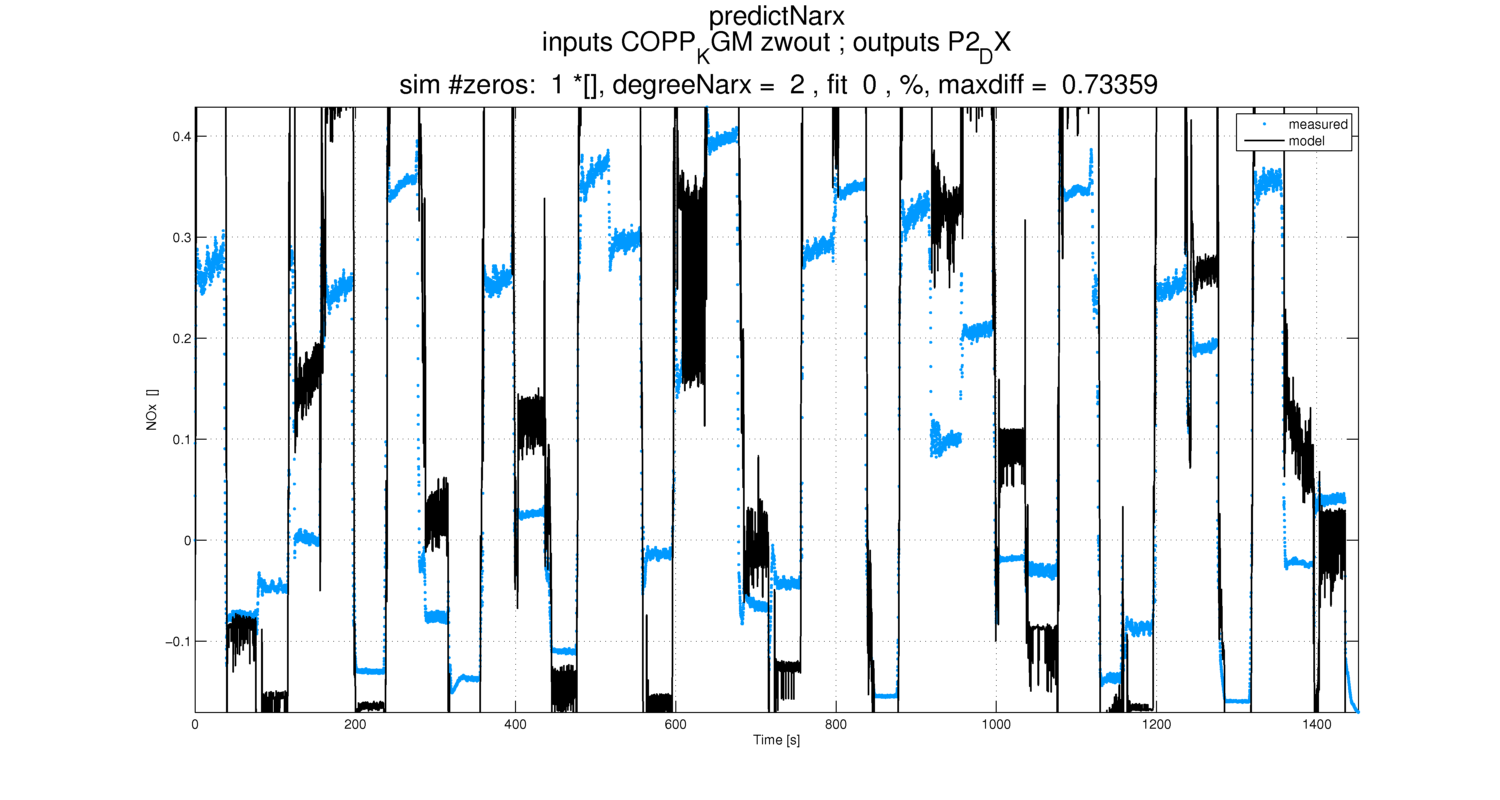
\includegraphics[width=.9\columnwidth]{Immagini/inputsCOPP_KGMzwoutoutputsP2_DX-predictNarx-3}
		\label{fig:inputsCOPP_KGMzwoutoutputsP2_DX-predictNarx-3}
	}
	\\
	\subfloat[P2 DX: Narx simulation]{
		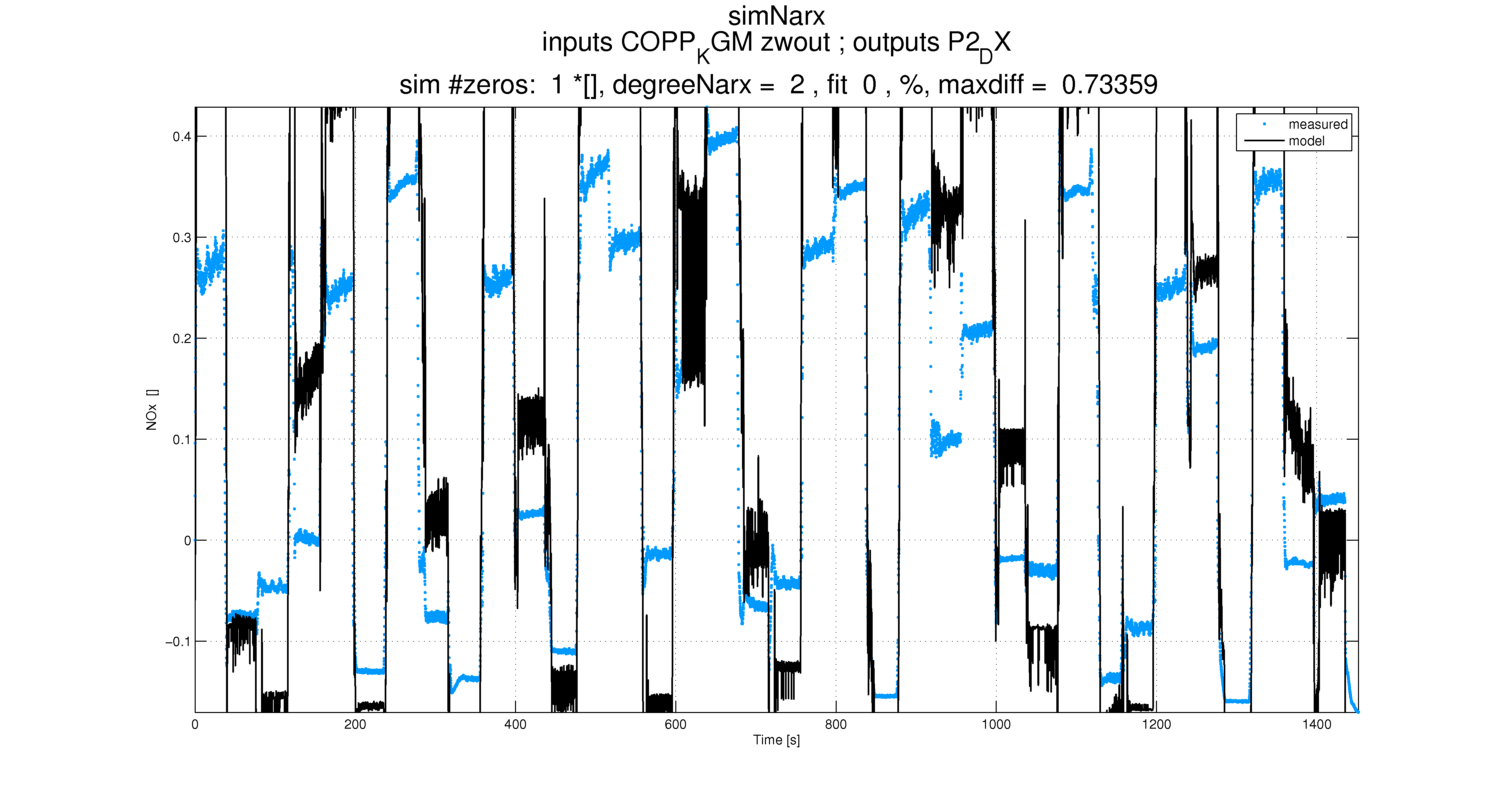
\includegraphics[width=.96\columnwidth]{Immagini/inputsCOPP_KGMzwoutoutputsP2_DX-simNarx-3}
		\label{fig:inputsCOPP_KGMzwoutoutputsP2_DX-simNarx-3}
	}
\phantomcaption	

\end{figure}


\begin{figure}[htbp] \ContinuedFloat
	\centering 
	\subfloat[P2 DX: Transfer function identification]{
		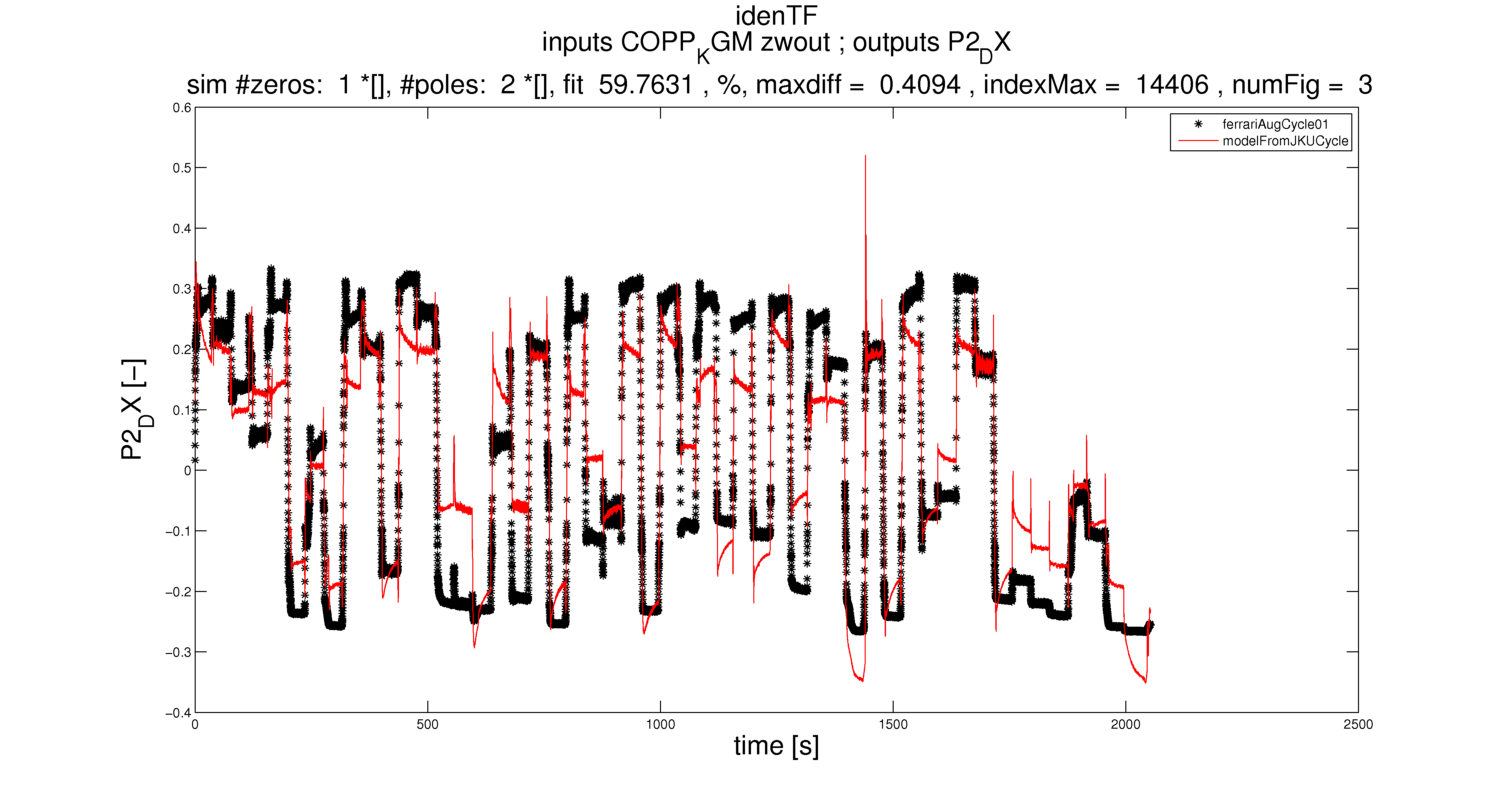
\includegraphics[width=.9\columnwidth]{Immagini/inputsCOPP_KGMzwoutoutputsP2_DX-idenTF-3}
		\label{fig:inputsCOPP_KGMzwoutoutputsP2_DX-idenTF-3}  }
	\\
	\subfloat[P2 DX: Transfer function simulation]{
		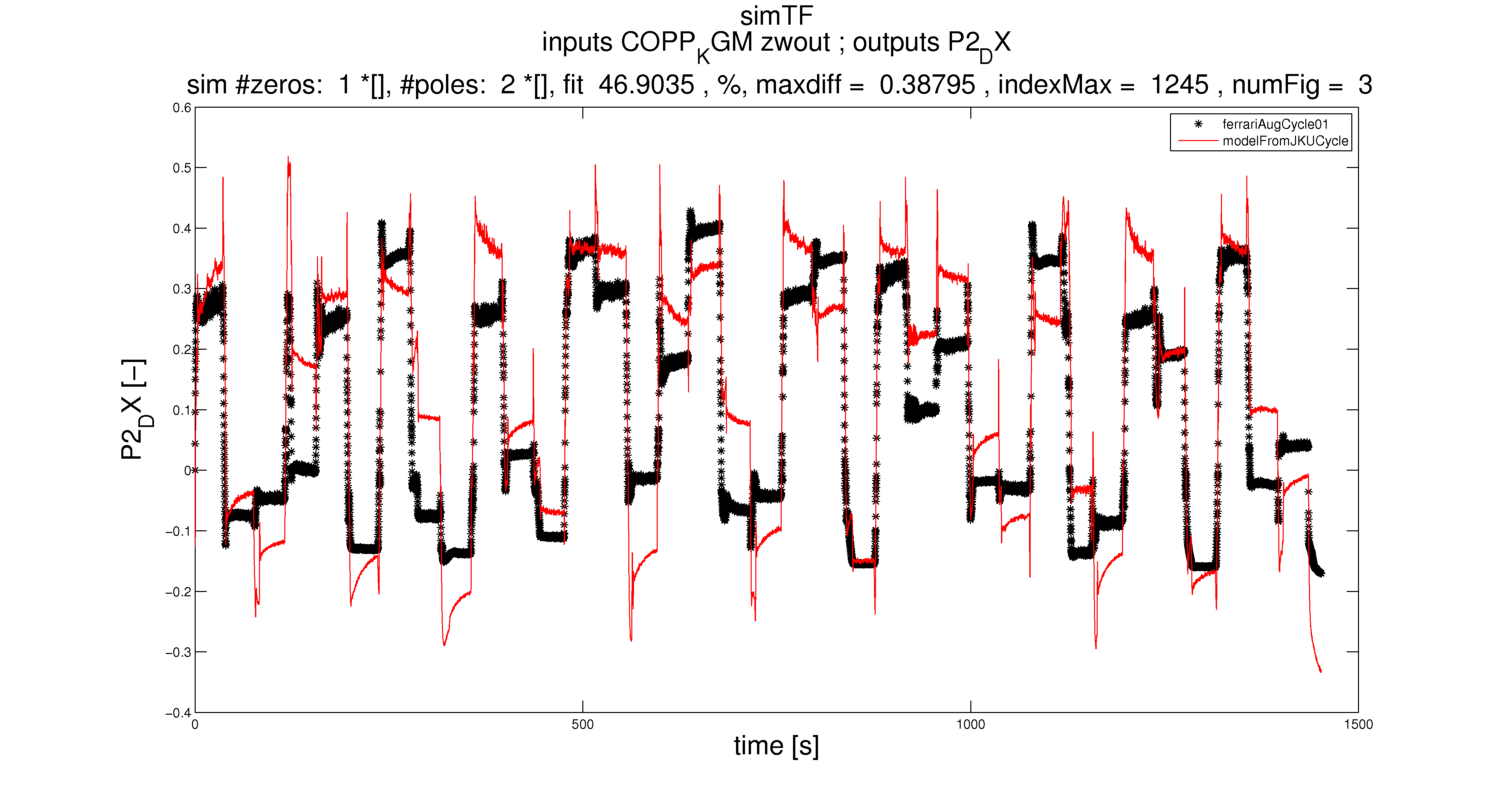
\includegraphics[width=.9\columnwidth]{Immagini/inputsCOPP_KGMzwoutoutputsP2_DX-simTF-3}
		\label{fig:inputsCOPP_KGMzwoutoutputsP2_DX-simTF-3}  }
	\\	
	\caption[Inputs: COPP KGM, zwout; Output: P2DX; np: 2; nz: 1; degree: 2]{Inputs: COPP KGM, zwout; Output: P2DX; np: 2; nz: 1; degree: 2}
	\label{fig:inputsCOPP_KGM-zwout-outputsP2_DX-3}	
\end{figure}